\cleardoublepage
\appendix

\chapter{Logging practice in software engineering}
Providing a guide for software engineers and developers to implement a suitable logging implementation in their software systems has to prove to be a vital tool in both industrial use and progress of academia \cite{Rong2018a}. Guoping Rong et al.~made a study to review these logging practices published papers to improve the performance and efficiency of logging implementation. From his study he made selection criteria to include (as in \Cref{tbl:CH1_RongIncSelectionCriteria}) and exclude (as in \Cref{tbl:CH1_RongExlSelectionCriteria}) academic papers about logging practices \cite{Rong2018a,Rong2018}.\par The Rong's selection criteria obtained numerous research papers of logging practices applied in the industry by either creating a new logging mechanism or optimising existing logging mechanisms. By reviewing 41 identified papers he found that many practitioners and researchers recognise the importance of logging practice in software engineering. There is a lack of guidance to provide software engineers or developers to create or improve their efficient logging mechanisms \cite{Rong2018a,Zhu2015}. 

\begin{table}[!htb]
	\centering
	\caption[G. Rong's inclusion selection criteria]
	{\textit{G. Rong's inclusion selection criteria \cite{Rong2018a}}}
	\label{tbl:CH1_RongIncSelectionCriteria}
	\begin{tabularx}{\textwidth}{|c|X|}
		\hline \textbf{Identification} & \textbf{Criteria} \\
		\hline I1. & Publications that investigate the methodology for logging practice. \\
		\hline I2. & Publications that investigate the tools, frameworks, systems which support logging practice. \\
		\hline I3. & Publications that propose a standard for logging practice.\\
		\hline I4. & Publications that are peer-reviewed (conference paper, journal article). \\
		\hline I5. & Publications that are primary studies on logging practice. \\
		\hline
	\end{tabularx}
\end{table}

\begin{table}[!htb]
	\centering
	\caption[G. Rong's exclusion selection criteria]
	{\textit{G. Rong's exclusion selection criteria \cite{Rong2018a}}}
	\label{tbl:CH1_RongExlSelectionCriteria}
	\begin{tabularx}{\textwidth}{|c|X|}
		\hline \textbf{Identification} & \textbf{Criteria} \\
		\hline E1. & Publications that investigate log analysis. \\
		\hline E2. & Publications that investigate the usage of logs. \\
		\hline E3. & Publications that investigate the technologies on logging user behaviours. \\
		\hline E4. & Publications that are not written in English. \\
		\hline E5. & Additionally, short papers, demo or industry publications are excluded. \\
		\hline
	\end{tabularx}
\end{table}

\clearpage

In \Cref{fig:PushblisedPapers} shows the distribution of the 41 published papers obtained for Rong's research relating to logging practices. Event logging has an increasingly important role in modern software systems, therefore the research focus on logging practices in software engineering have been on a rise between 1990 and 2017.

\begin{figure}[!htb] % An h :here, t: top, b: bottom.
	\centering % cent the figure
	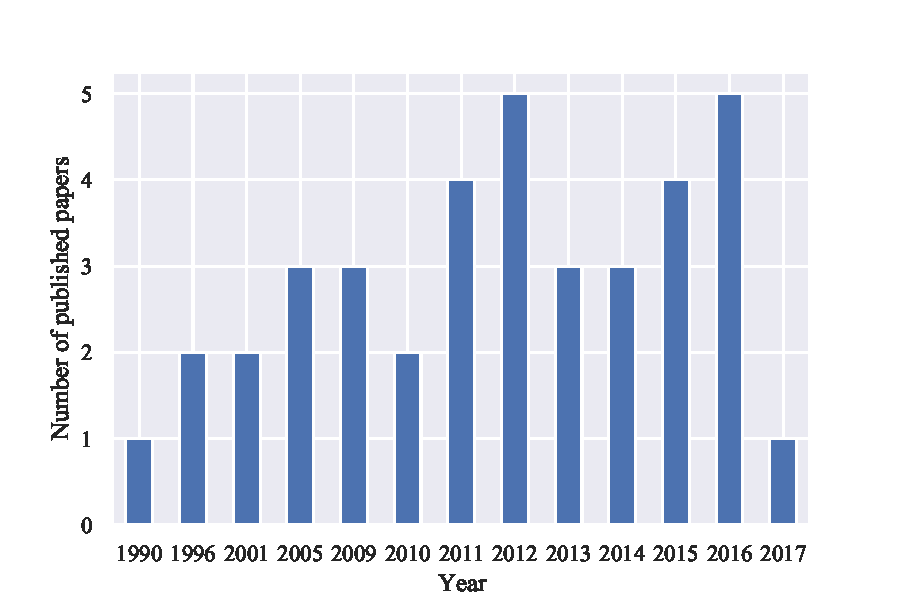
\includegraphics[width=0.95\textwidth]{Chapter1/Ronga2018.pdf}
	\caption[The distribution of the papers’ published years]
	{\textit{The distribution of the papers’ published years \cite{Rong2018a}}} \label{fig:PushblisedPapers}
\end{figure} 

\chapter{Software maintenance model}
%TODO Example maybe not relevant
A software maintenance model is an abstract representation of software systems' evolution to keep track of all the maintenance activities when implementing software maintenance \cite{Ren2011}. The \textit{IEEE Standard 1219} for software maintenance is the standard that should be followed when planning software maintenance as in \Cref{fig:ch1_ieeeModel}.\par It is crucial to identify the maintenance that should be done before making, which will start with the user or developer's request to modify the software. A feasibility analysis of any changes that are required is made. A certain amount of resources will be needed to implement maintenance, and this will impact the design and implementation phase. System and acceptance testing are essential to ensure that the system is still fully functional. After the system is thoroughly tested and approved, it will be available to the user, and the maintenance process will start again when there are new improvements made to the software system.

\begin{figure}[!htb] % An h :here, t: top, b: bottom.
	\centering % cent the figure
	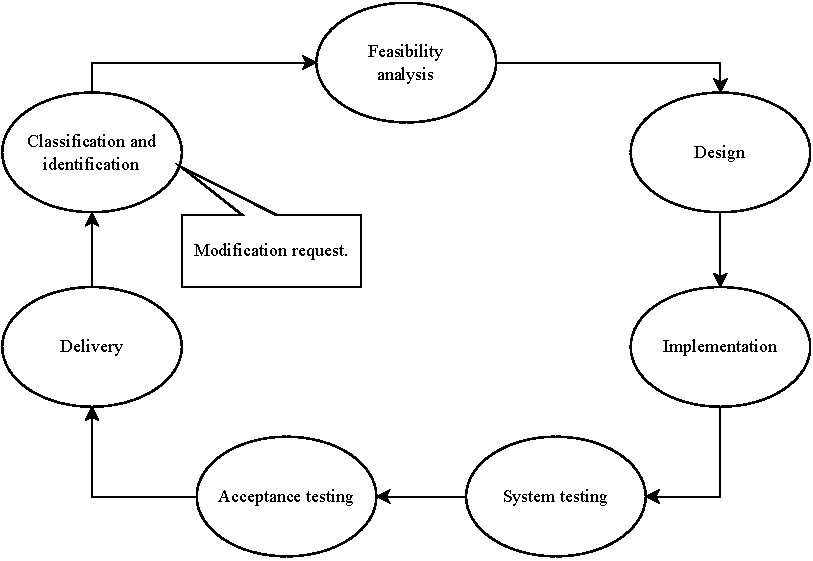
\includegraphics[width=0.6\textwidth]{Chapter1/IEEE_Model/IEEE_Model.pdf}
	\caption[IEEE model]
	{\textit{IEEE model \cite{Ren2011}}} \label{fig:ch1_ieeeModel}
\end{figure}

Most organisations' maintenance models will be based on \Cref{fig:ch1_ieeeModel} to manage their maintenance efforts. About $50\%$ of the developer implementing maintenance job is to understand what the software system is supposed to do, and the changes they make will not change the intended functionality of the system \cite{Tang2010, Zhuo1993}. This is due to the problems with implementing maintenance as discussed in \Cref{sec:ch1_maintenanceProblems}.\par \Cref{fig:ch1_maintenanceFlow} example of what a practical maintenance flow model an organisation would likely use to implement software maintenance. Initially, a developer will complete a request form or issue indicating a new problem or feature request that needs to be implemented \cite{Tang2010}.\par If the issue is a problem in the software system, the severity of the problem needs to assess to decide on the priority level to resolve it. This type of maintenance is mostly corrective and can also be preventive if it is a possible solution to prevent any software failures in the future \cite{Tang2010}. Other types of maintenance requests are either adaptive or perfective and usually placed in the development team's task queue.\par After all the maintenance tasks are defined, the development team will prioritise the higher-rated issues that need to be solved. This process will repeat itself until all the task for that specific software system is completed.\par To fully follow the \textit{IEEE Standard 1219} of implementing maintenance on a software system, the defects or areas of improvement are identified. Utilisation analysis of event logs can be used to detect any hidden defects or performance issues in a software system to implement software maintenance \cite{Cinque2013, Rong2018a, Levin2019}.

\begin{figure}[!htb] % An h :here, t: top, b: bottom.
	\centering % cent the figure
	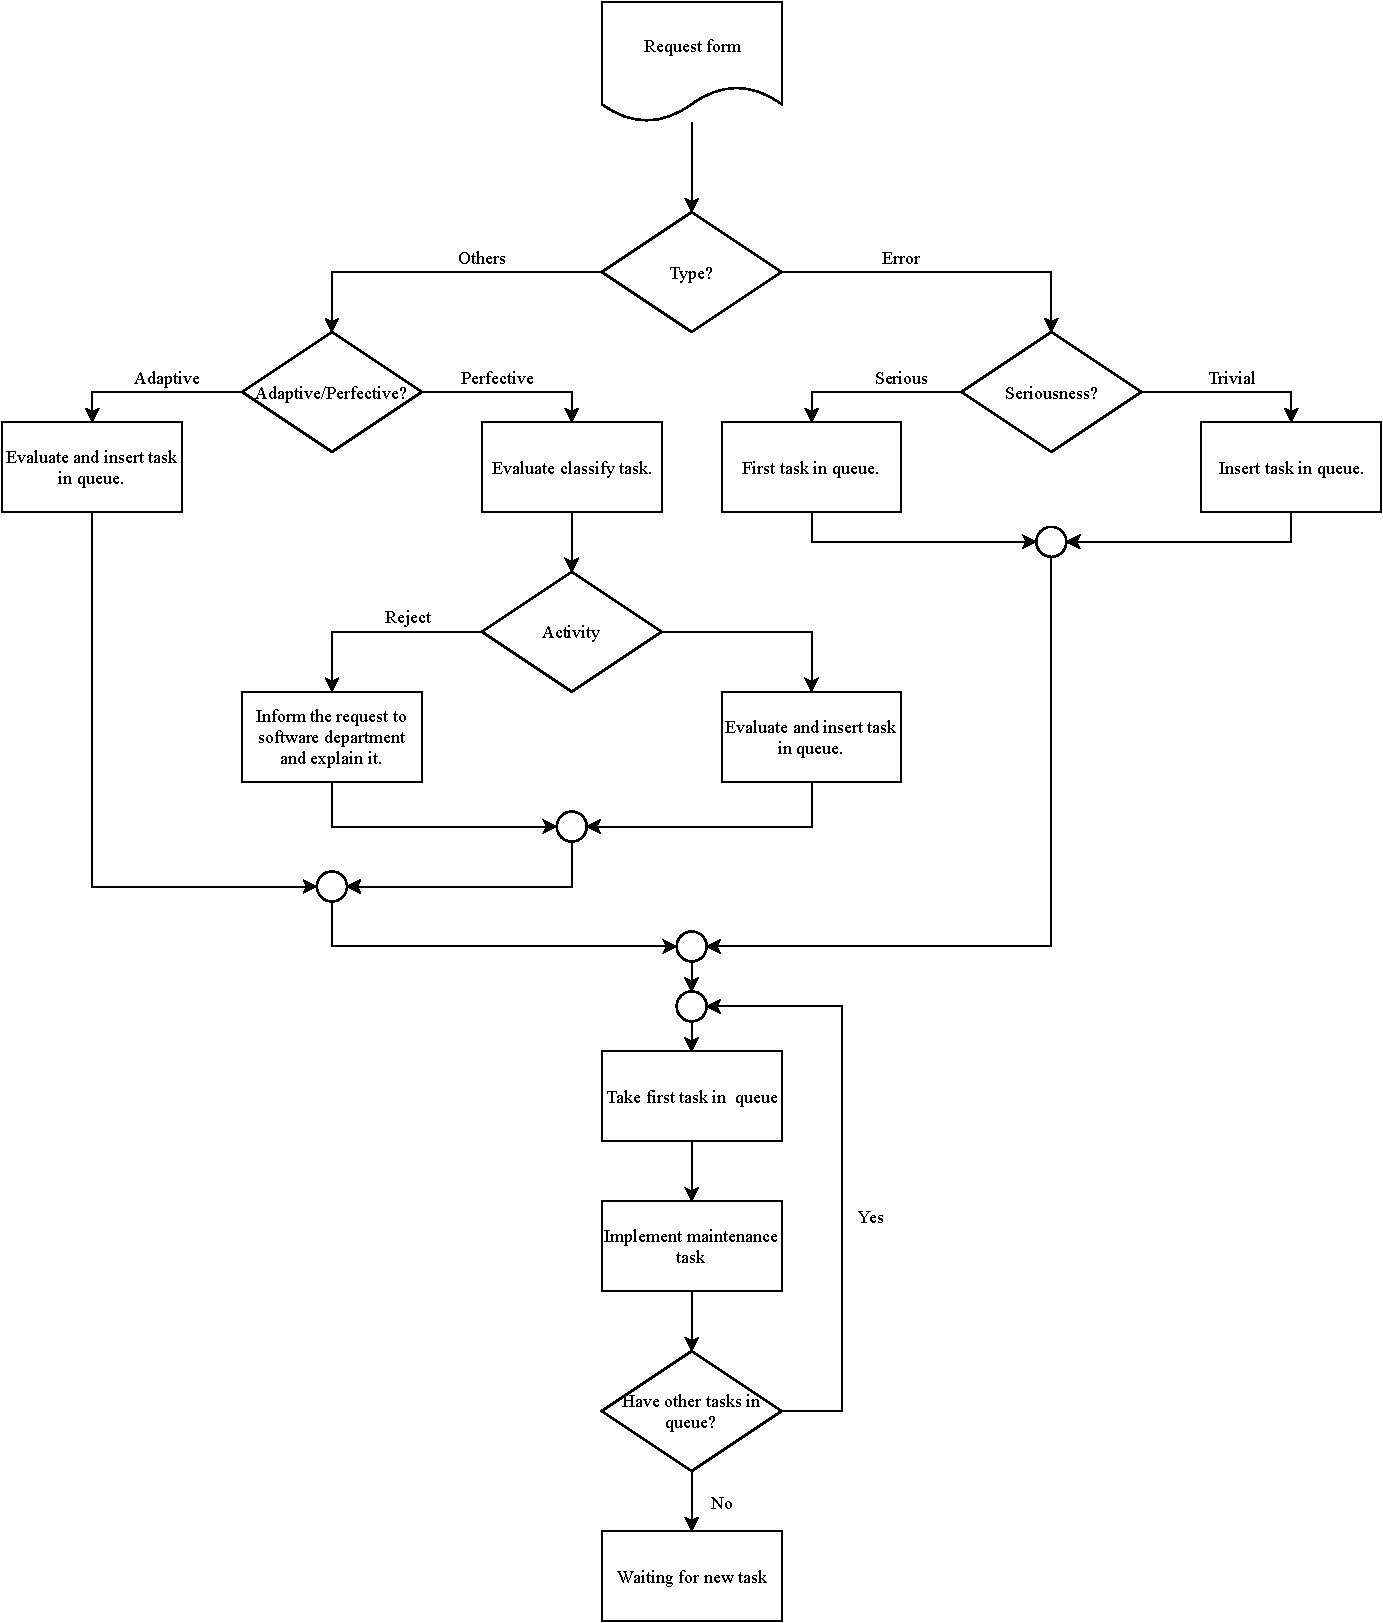
\includegraphics[width=0.85\textwidth]{Chapter1/Maintenance_flow/Maintenance_Flow.pdf}
	\caption[Maintenance flow model]
	{\textit{Maintenance flow model \cite{Tang2010}}} \label{fig:ch1_maintenanceFlow}
\end{figure}
